\chapter{Resultat}
Det här kapitlet kommer att beskriva resultatet av den mjukvaran som har utvecklats samt vilka erfarenheter som
teamet har samlat på sig under projektets gång.

\section{Systembeskrivning}
Systemet som skapats består av två separata delar, en back-end och en front-end.

\subsection{Front-end}
Projektets front-end utvecklades i ramverket Angular. Front-end använder sig därför av den komponentbaserade arkitektur som starkt förordas av ramverket. Systemets front-end använder Angulars arkitektur för att implementera designmönstret MVC (se \ref{mvc-ref}).

Det grafiska innehållet på projektets front-end är uppdelat i komponenter som uppdateras eller byts ut till andra komponenter när användaren interagerar med systemet. De komponenter som finns överst i applikationens komponenthierarki är tomma behållare vars enda syfte är att separera applikationens olika beståndsdelar från varandra. Inuti dessa har sedan komponenter med faktiska funktioner, som knappsatser eller sökrutor, placerats.

Applikationen består av flera olika vyer, där vissa av vyerna ska visas upp i samma behållare men vid olika tillfällen, beroende på vilken vy användaren för stunden är intresserad av. För att byta mellan vyerna används Angulars tjänster. Tjänsterna är inte direkt kopplade till någon specifik komponent och används därför för att kommunicera mellan komponenter i olika delar av komponenthierarkin.

All den data om patienter, salar och utrustning som användaren är intresserad av finns på en server i projektets back-end. Därför är det nödvändigt med kommunikation mellan de båda delarna. På projektets front-end sköts kommunikationen med AJAX-anrop. Dessa anrop sker i tjänster för att de ska vara tillgängliga för alla komponenter som behöver tillgång till data av olika sorter.

\subsection{Back-end}
Back-end i projektet är en server som har två huvuduppgifter. Den första är att vara värd för klienten så att den kan kommas åt av flera användare och datorer över nätverk. Den andra uppgiften är att ha en databas med tillhörande webb-API. Databasen används för att hantera all data som behövs för schemaläggningen som bland annat operationsbeslut, kirurger, resurser och bokningar med mera. Webb-API tillåter klienten att kunna logga in och sedan hämta och modifiera denna data.

Servern är byggd på miljön Node.js och är skriven i JavaScript. Den använder sig av Node.js-biblioteket Express för den statiska leveransen och klienten och för att definiera HTTP-API:t. För hantering av databasen används i grunden MySQL men även ORM-biblioteket Sequelize i Node.js. Sequelize tillåter objekt-orienterad hantering av databasen och tar bort behovet att använda direkta SQL-frågor. All test-data som används i prototypen läggs också in i databasen med hjälp av seeds i Sequelize. Mer om seeds och Sequelize går att läsa i stycke \ref{sec:sequelize_teori} i teorin.

Hela API:t i servern skyddas bakom autentisering. Detta görs med hjälp av Node.js-biblioteket Passport och ser till att ingen data i databasen kan kommas åt eller modifieras utan att först logga in.

\subsection{LoFi-Prototyper}

\begin{figure}[H]
  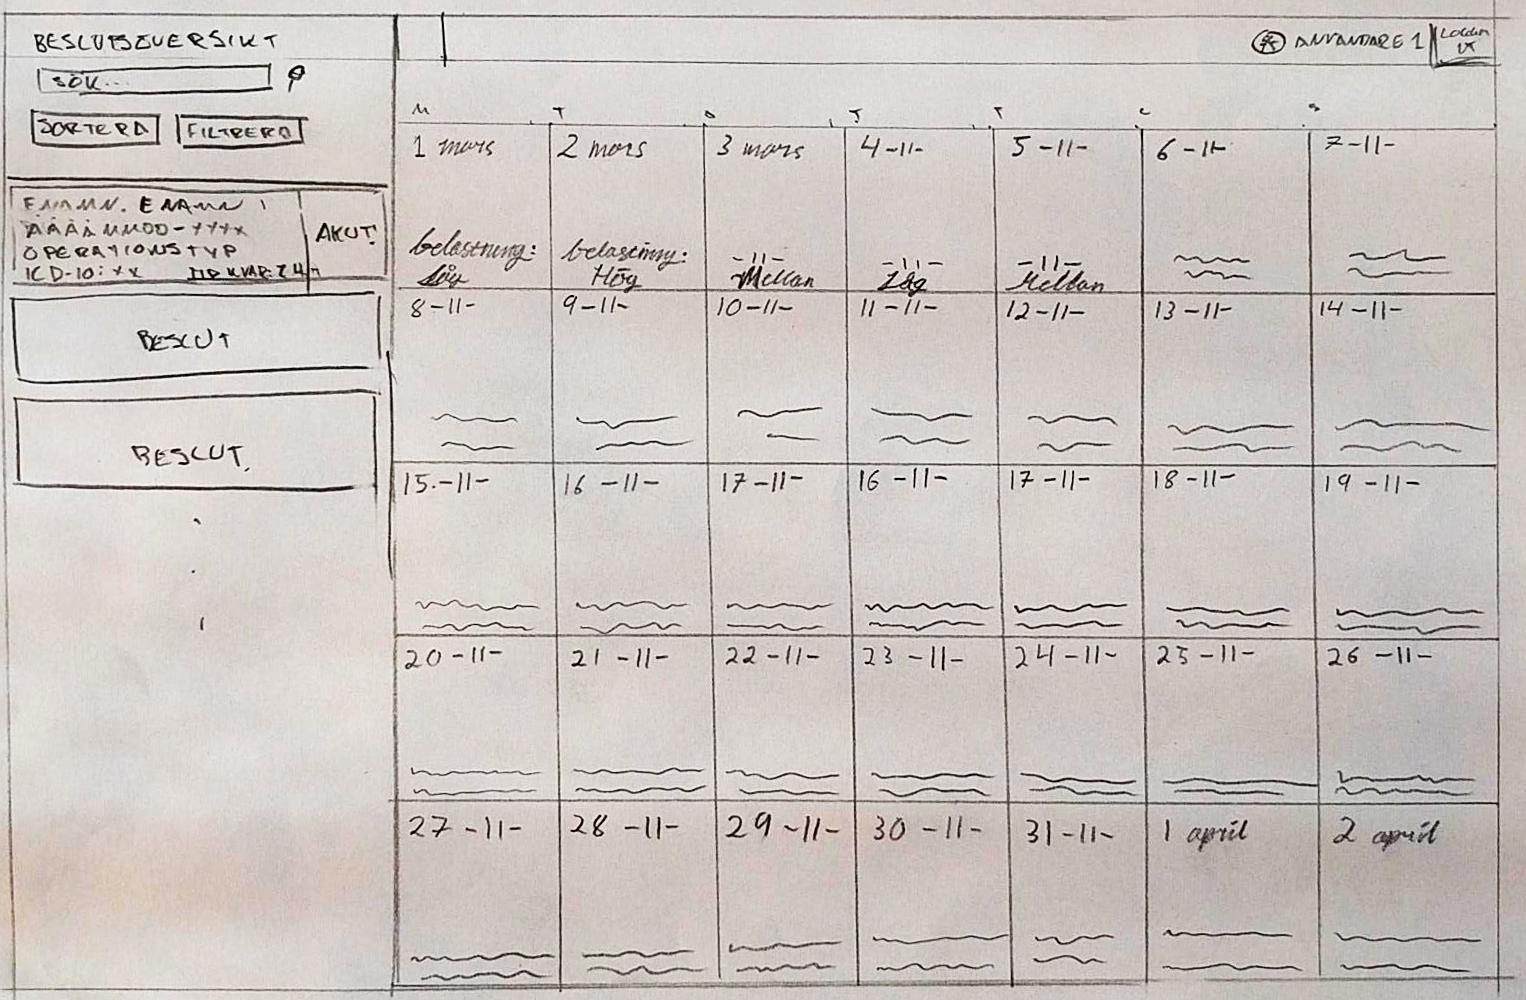
\includegraphics[width=\linewidth]{Figures/LoFi_no2.jpg}
  \caption{Sista LoFi-prototypen}
  \label{fig:LofiPic}
\end{figure}


Under projektets andra iteration utvecklades tre olika LoFi-prototyper. Dessa
LoFi-prototyper designades för att visa på olika designalternativ på
användargränssnittet. Ett exempel på detta är informationen som var med i listan
över beslutade operationer.

I en av prototyperna identifierades patienten som hörde ihop med beslutet med namn, den andra med personnummer. I den tredje LoFi-prototypen
fanns inget som identifierade patienten utan enbart information om vilken
typ av operation det var. På liknande sätt utvärderades olika sätt att
visualisera lediga tider i schemat samt olika sätt att anpassa sökparametrarna för en sökning efter lediga tider.

När prototyperna visades för kunden kunde alternativen sållas bort och en tydligare bild av behoven framträdde.
Till exempel fanns det endast personnummer och inte namn på patienterna, vilket var något som önskades.

Den första iterationen av LoFi-prototyper användes sedan för att ta fram en ny
LoFi-prototyp med enbart mindre designalternativ som visades för tre olika
operationsplanerare. (Figur \ref{fig:LofiPic} illustrerar en bild av den sista Lofi-prototypen.)

\subsection{Grafiskt gränssnitt}
Då arbetet med prototyper var klart inleddes implementationen av designen i form av de grafiska komponenterna. Det här resulterade i en komplett webbsida med tre olika huvudkomponenter, sidopanelen, informationslisten och den huvudsakliga innehållsrutan.

Arbetsflödet i appen börjar med att användaren loggar in med sina inloggningsuppgifter. Därefter presenteras vyn som visas i figur \ref{fig:window}.

\begin{figure}
	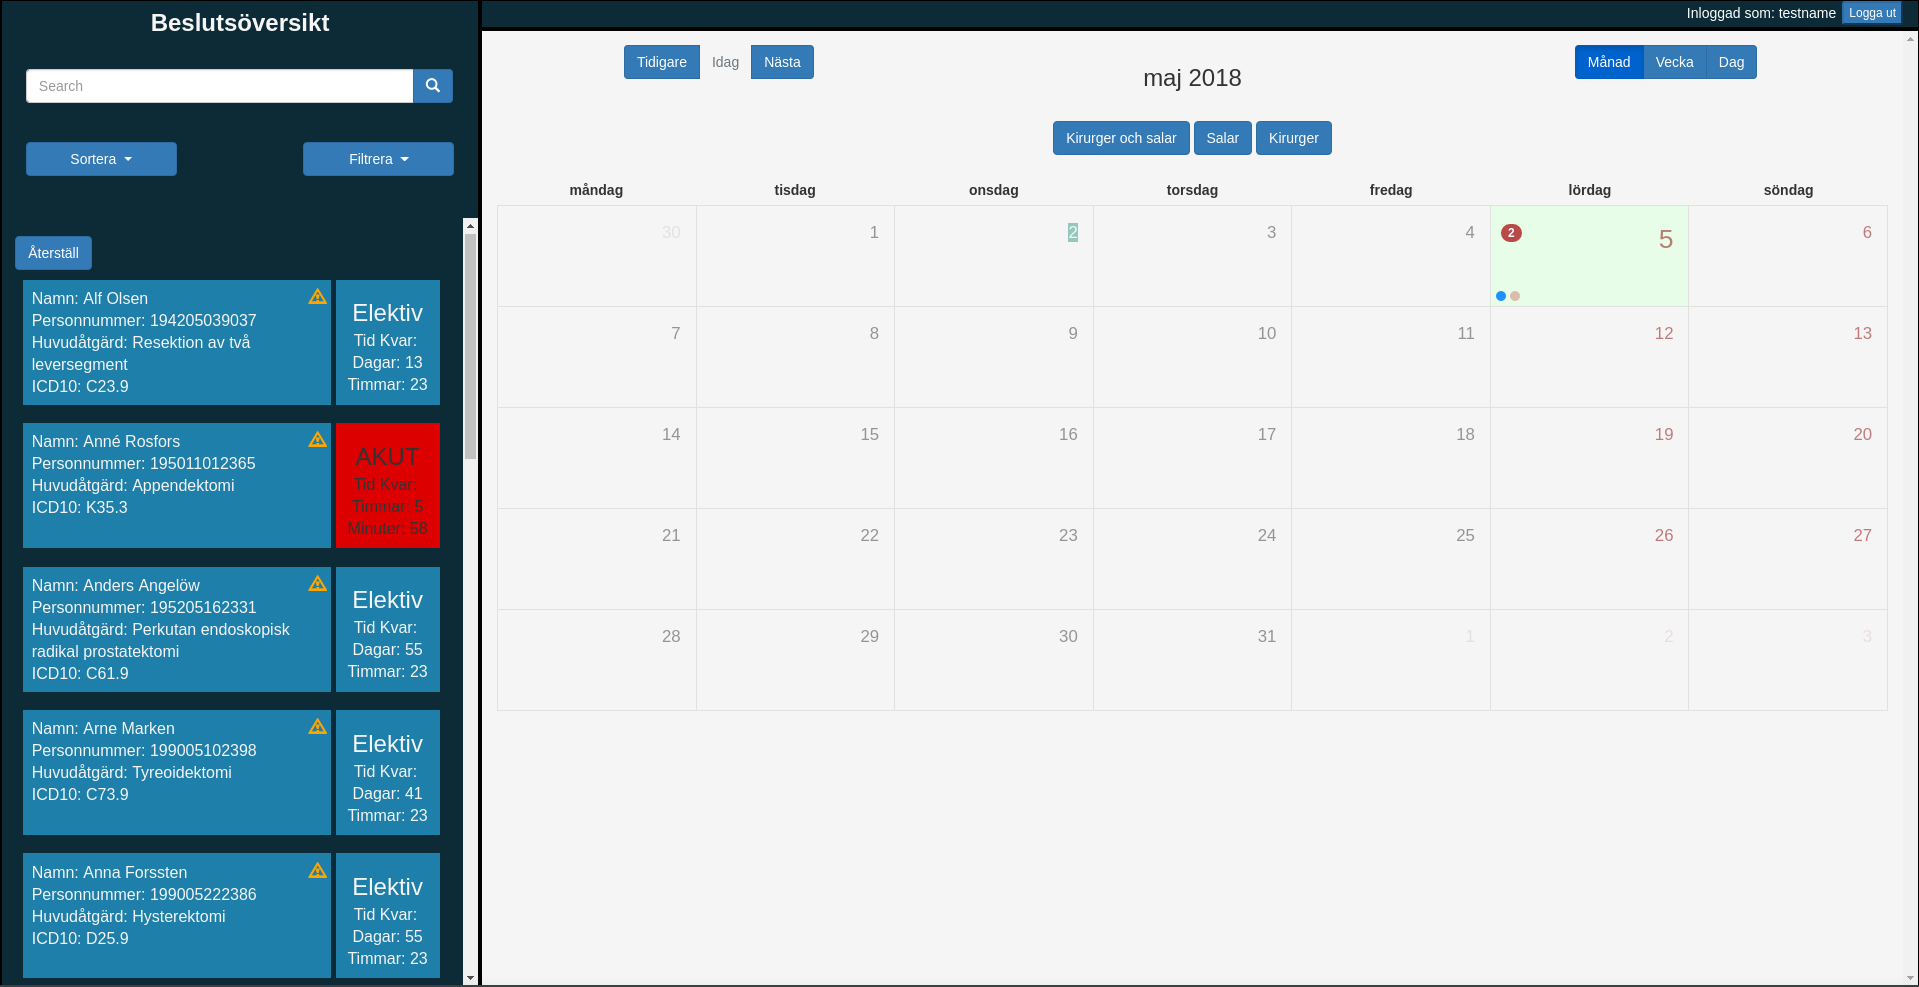
\includegraphics[width=\linewidth]{Figures/window.png}
	\caption{Gränssnittet}
	\label{fig:window}
\end{figure}


\subsubsection{Sidopanelen}
När användaren loggat in så pressenterar sidopanelen alla de beslut som finns att planera (figur \ref{fig:beslutsvy}). Ett beslut visuliseras som ett kort som innehåller en mängd viktig data så som patientens namn, personnummer, hur långt det är innan operationen bör ske och även vilken typ av operation det gäller samt vad anledningen är till att operationen behövs. En akut operation är tydligt markerad med rött för att det enkelt ska gå att se att det är viktigt att boka in denna så snart som möjligt.

Det går även att söka i listan dessutom kan användare filtrera listan på olika kriterier samt sortera den.

När användaren klickar på en patient så visas en detaljvy för patienten (figur \ref{fig:planeringsvy}). Här kan användaren se mer detaljerad information om beslutet så som hur lång tid operationen beräknas ta, hur lång förberedelse tid som krävs mm. Det går ochså att se en lista med alla de verktyg och matrial som krävs.

Längst ner finns det även en ruta med sökkriterier för att filtrera den schemavy som visas i huvudfönstret så att en ledig tid kan hittas.
\begin{figure}[H]
	\centering

	\begin{subfigure}[b]{0.4\linewidth}
		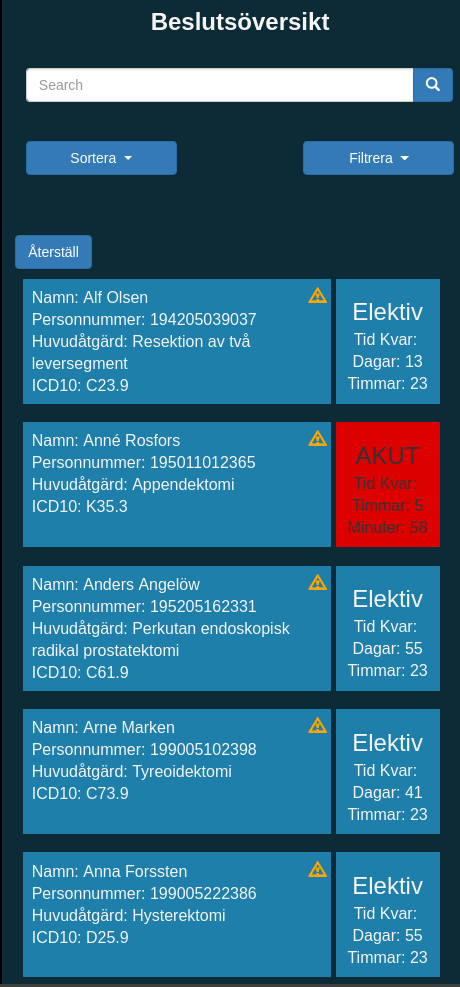
\includegraphics[width=\linewidth]{Figures/beslut.png}
		\caption{Beslutsvyn}
		\label{fig:beslutsvy}
	\end{subfigure}
	\begin{subfigure}[b]{0.4\linewidth}
		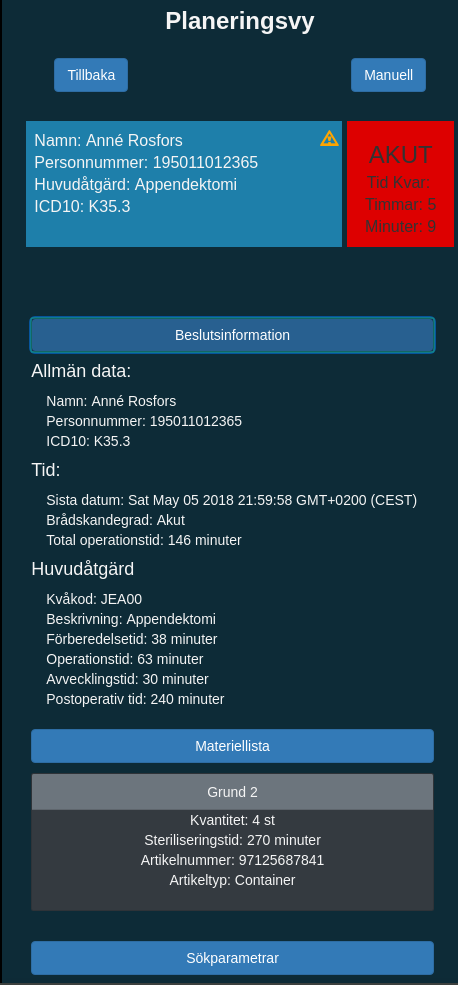
\includegraphics[width=\linewidth]{Figures/planning.png}
		\caption{Planneringsvyn}
		\label{fig:planeringsvy}
	\end{subfigure}
	\caption{Sidopanelens två vyer.}
	\label{fig:sidepanel}
\end{figure}


\subsubsection{Informationslisten}
Informationslisten är till för att alltid visa information om den patient som för tillfället håller på att bokas in. Så snart ett beslut har valts i sidopanelen så visas patientens namn och personnummer i informationslisten.

I informationslisten syns det också vilken användare som är inloggad längst till höger och det finns även en knapp för att logga ur aktuell användare.

\subsubsection{Huvudfönstret}
I huvudfönstret visas i grundutförandet en månadsvy över där det går att se hur många operationer det är inbokade på olika dagar. Om en dag markeras så visas fler detaljer över de operationer som är inbokade på den dagen. När en patient har valts i sidomenyn används måndadsvyn för att välja vilken dag då man vill boka in operationen. När en dag har valts så skickas användaren vidare till spårvyn.

\subsubsection{Spårvyn}
Spårvyn visar ett antal konfigurerbara spår där varje spår motsvarar schemat för en viss resurs på den valda dagen. Dessa spår visas brevid varandra för att enkelt visualisera de olika resurserna och på så sätt skapa en bra överblick över när de olika resurserna är lediga i relation till varandra. Det går att välja vilka resurser som ska visas så som salar, olika personal och verktyg. \todo{Utöka med vidare förklaring när den är fastställd.}\todo{infoga bild på spårvy}



\subsection{Systemanatomi}
I första iterationen togs det fram en systemanatomi (se figur \ref{fig:Systemanatomi}) som användes under projektets gång som ett hjälpmedel för att strukturera upp arbetet under utvecklingen. Den gav en översiktlig bild av vilken funktionalitet produkten skulle innehålla och hur de olika delarna samverkade med varandra. Utöver detta presenterades den i ett tidigt skede för kunden i syfte att säkerställa att projektgruppens syn på systemet stämde överens med kundens.

\begin{figure}[H]
    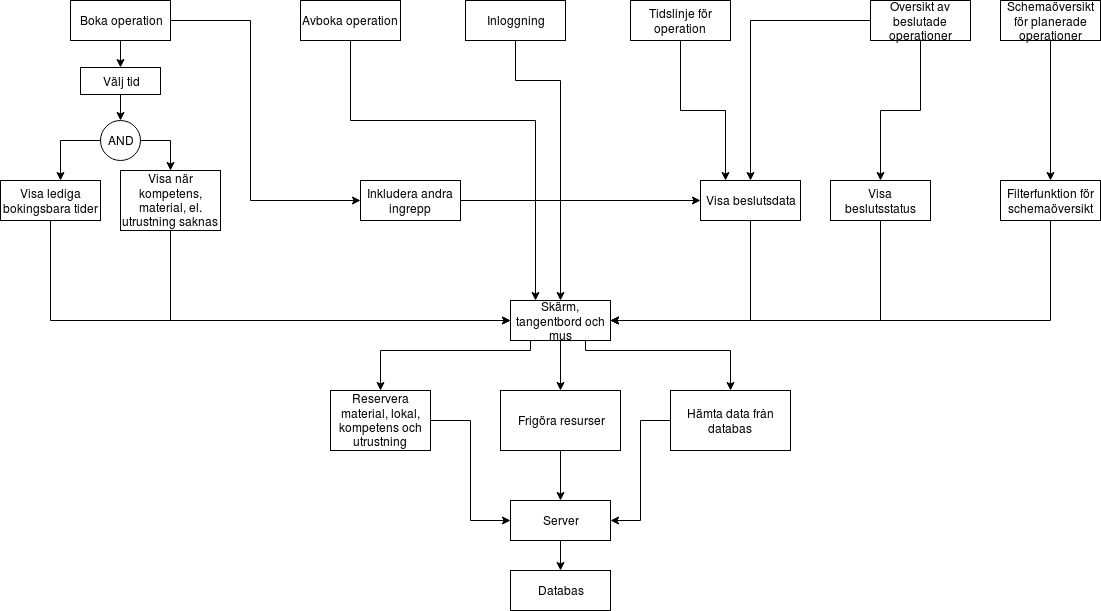
\includegraphics[width=\textwidth,height=.4\textheight]{Figures/Systemanatomi.png}\\
    \caption{Systemanatomi}
    \label{fig:Systemanatomi}
\end{figure}

\subsection{Värde för kund}
Den produkt som har skapats är ett lättöverskådligt schemaläggningssystem för operationer. Systemet matchar väl med den initila målbilden. Sedan har nya upptäckter under projektets gång gjort att systemet förmodligen behöver kompleteras avsevärt för att vara praktiskt användbart. Detta är dock inte ett stort problem då syftet var att skapa en prototyp (se stycke \ref{sec:syfte}).

Dokumentationen och processen under projetket har varit minst lika viktig i att ta reda på vad som kommer och inte kommer att fungera och ger stor insikt i hur systemet kan se ut och hur produkten kan förbättras i framtiden.

Vår förhoppning är att de arbetsdokument som vi tagit fram i gruppen som stöd under arbetet vara till hjälp för den fortsatta utvecklingen. Detta tillsammans med de officiella dokumenten borde skapa en solid teoretisk kunskapsgrund för vidareutveckling.

Vad gäller faktiskt programvara så tror vi starkt på att det finns funktioner och element i vår design som bidrar med en ny syn på schemaläggning och som kan komma till användning antigen så som vi implementerat dem eller att de kan vara till inspiration för andra nya sätt att bygga upp systemet.

Totalt sett medför detta att Region Östergötland kommer att ha en bra grund att utgå ifrån då deras projekt startar. Både projekledaren och andra aktörer för det större projetket kommer att kunna ta med sig många erfarenheter från det här projekt i och med att flera av dem har varit så delaktiga i vår process genom flera möten.

\section{Gemensamma erfarenheter}
Under projektet har medlemmarna fått stor erfarenhet av webbprogrammering då ingen hade någon större erfarenhet av detta sedan tidigare. Gruppen har fått sätta sig in i HTTP-protokoll, databaser och ett flertal programspråk och ramverk. Även versionshantering med git och gitlab har gruppen fått fördjupad kunskap inom.

Vid utveckling av front-end lärde sig gruppen att använda ramverket Angular och att programmera i HTML, CSS och TypeScript. I back-end behövde medlemmarna istället sätta sig in i JavaScript, MySQL-databaser och miljön Node.js med ett flertal tillhörande bibliotek.

Förutom tekniska erfarenheter har gruppen fått en större förståelse för hur sjukvården fungerar och att ett bra IT-system kan göra stor verklig skillnad. Gruppen har även fått praktiskt erfarenhet av att utöva Scrum. Det har varit seminarier där presentation och opponering ingick.

Slutligen så har de fått kunskap att utveckla något i grupp, där förkunskaper saknades eller var begränsade och som införskaffas allteftersom.

\section{Översikt över individuella bidrag}
I denna delen presenteras deltagarnas individuella bidrag översiktligt.

\todo{Lägg till era rubriker och en kort synopsis här}
\subsection{Adam}
En studie i hur teamledarens roll går att applicera tillsammans med scrum-metodik.
\subsection{Björn}
Hur kan versionshantering användas effektivt för ett mindre mjukvaruutvecklings projekt.
\subsection{Christoffer}
Betydelsen av att samla krav från en varierad grupp aktörer
\subsection{Jämförelse mellan TypeScript och JavaScript av Henrik Lindström}
Denna rapport jämför språken TypeScript och JavaScript baserat på erfarenheter från projektet och litteratur. Undersökningen fokuserar på TypeScript och JavaScripts olika typsystem, statiskt typning och dynamisk. Inom detta är det påverkan på feldetektering, kodförsåelse och produktivitet med de två systemen som behandlas.
\subsection{Martin}
Angular som webbutvecklingsplattform
\subsection{Niclas}
Prototypuveckling i kandidatprojekt
\subsection{Tor}
Kvalitetsförsäkrande metoder i ett småskaligt mjukvaruprojekt
